\documentclass{article}

\usepackage{amsmath}
\usepackage{amssymb}
\usepackage[spanish]{babel}
\usepackage[margin=1.5in]{geometry}
\usepackage{graphicx}
\usepackage[utf8]{inputenc}

\renewcommand{\Bbb}{\mathbb}

\begin{document} 

\section{EDO - clase 1}

Una función escalar es diferenciable si y sólo si se puede escribir lo siguiente:

\begin{equation}
f(x+h) - f(x) = f'(x) h + \mu(h) h
\end{equation}

En el lado derecho de esta igualdad, el primer sumando es el \textbf{diferencial total de la función}, y el segundo es un infinitésimo que tiende a cero cuando h tiende a cero.

Propiedades:

\begin{subequations}
\begin{align}
d k & = 0 \\
d(k f) & = k df \\
d(f \pm g) & = df \pm dg \\
d(f g), d( f / g ) & = \textbf{igual que derivada} \\
dy & = f'(x) h \wedge h = dx \Longrightarrow y' = \frac{dy}{dx} = f'(x)
\end{align}
\end{subequations}

Esta última se conoce como la notación de Leibnitz.

Una ecuación diferencial, o ED, es una ecuación donde las incógnitas son funciones; toda ED relaciona una función a determinar, su(s) variable(s) independiente(s), y las derivadas de la función. Las EDs pueden ser:

//TODO Usar bullet list
* Ordinarias: La función incógnita tiene una sola variable independiente.

* En derivadas parciales: La función incógnita tiene más de una variable independiente.


\subsection{Orden de una ED}

El orden de una ED está dado por la derivada de mayor orden de la función incógnita.

\subsection{Expresión general}

Expresión general orden 1:

\begin{equation}
F(x, y, y') = 0
\end{equation}

Normalizada orden 1:

\begin{equation}
y' = g(x, y)
\end{equation}

Expresión general para orden N:

\begin{equation}
F(x, y, y', y'', ..., y^(n)) = 0
\end{equation}

Se dice que $x, y, y', ..., y^(n)$ son las variables de la ED $F$.

\subsection{Grado de una ED}

Aquellas ED que pueden expresarse como polinomios respecto al orden de las derivadas, y donde además los coeficientes que multiplican a las derivadas son constantes o funciones de $x$, tienen \textbf{grado}. El mismo corresponde al exponente al que está elevada la derivada de mayor orden.

Si algún coeficiente depende de $y$, la ED no tiene grado.

\subsection{Soluciones de una ED}

Sea $y = g(x)$ una función definida en un intervalo $I$, con $n$ derivadas continuas en dicho intervalo. Si al reemplazar $y$ en una ED, la misma se reduce a una identidad, se dice que $y = g(x)$ es solución de la ED en $I$. En tal caso, $I$ es denominado intervalo de solidez, intervalo de existencia, o dominio de la solución.

\subsubsection{Solución general (SG)}

La SG de una ED de orden $n$ es una relación funcional entre sus variables 
que contiene $n$ constantes arbitrarias linealmente independientes.

\subsubsection{Solución particular (SP)}

Se obtiene a partir de la SG al darle valores concretos a sus constantes; usualmente, ello requiere $n$ valores iniciales o condiciones de contorno de la función incógnita y sus derivadas.

\subsubsection{Solución singular (SS)}

Una función es SS de una ED cuando la reduce a una identidad, pero no puede obtenerse a partir de una SG. No toda ED tiene SS.

\section{EDO - clase 2}

\subsection{Teorema Fundamental del Cálculo}

El TFC plantea que dos funciones $f$ y $g$, definidas en un mismo dominio, difieren en una constante $\Leftrightarrow$ sus derivadas son iguales. Esto implica que al resolver una integral, se obtiene siempre una familia de primitivas:

\begin{equation}
\int f(x) dx = F(x) + C \Leftrightarrow F'(x) = f(x)
\end{equation}

\subsection{Isoclinas y conjuntos de nivel}

Dada una familia de curvas, las isoclinas de nivel $k$ son las rectas (o curvas) que unen los segmentos tangentes de pendiente $k$. Simbólicamente:

\begin{equation}
y' = F(x,y) \Rightarrow I_k = {(x,y) \in Dom(F) / F(x,y) = k}
\end{equation}

Las isoclinas son las curvas de nivel de la función derivada.

\begin{figure}[t]
\caption{Isoclinas}
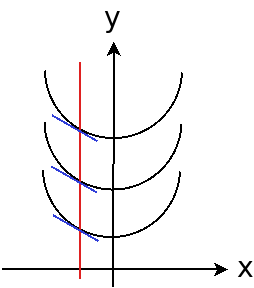
\includegraphics[scale=0.75]{img/edo_fig001_isoclinas.png} 
\centering
\label{fig:isoclinas}
\end{figure}

Por ejemplo, dada una familia de curvas parabólicas, obsérvese la figura ~\ref{fig:isoclinas} en los puntos donde la tangente (azul) es igual, se unen los puntos obteniendo una recta (rojo). Esa es la isoclina para ese valor en particular. Nótese que hay tantas curvas isoclinas como valores tome la derivada; en el gráfico se muestra una sola.

\subsection{Formando EDOs a partir de una familia de curvas}

Sea $F(x, y, C_1, C_2, ..., C_n)$ una familia de curvas. Habiendo $n$ constantes independientes entre sí, al derivar $F$ $n$ veces consecutivas surge un sistema de $n$ ecuaciones a partir del cual se podrá obtener una ecuación diferencial. Por ejemplo:

\begin{equation}
y = C_1 \cos(x) + C_2 \sin(x)
\end{equation}

Hay dos constantes independientes; por lo tanto, derivo dos veces respecto a $x$ miembro, planteando además que $y' = f'(x)$:

\begin{subequations}
\begin{align}
y' = -C_1 \sin(x) + C_2 \cos(x) \\
y'' = -C_1 \cos(x) - C_2 \sin(x)
\end{align}
\end{subequations}

Sumando las expresiones para $y$ e $y''$ miembro a miembro, se obtiene la ED $y + y'' = 0$

A veces, las constantes no son independientes entre sí, aunque lo parezcan. Por ejemplo:

\begin{equation}
y = A + \ln \left( \frac{B}{x} \right) \Rightarrow y = \ln C + \ln \left( \frac{B}{x} \right) = \ln \left( \frac{C B}{x} \right) = \ln \left( \frac{K}{x} \right)
\end{equation}

Así, lo que parecía de segundo orden, era de primer orden. Derivar una vez alcanza para obtener la ED:

\begin{equation}
y' = \frac{1}{\frac{K}{x}} -\frac{K}{x^2} \Rightarrow y' = \frac{-1}{x}
\end{equation}

Si una familia de curvas es solución pero está expresada implícitamente, puede que haya que determinar su dominio de validez.

\end{document} 
